%% GPs for classification and ordinal regression
\lecture{GPs for classification and ordinal regression}{Classification}

\begin{frame}
	\frametitle{GPs for Classification and ordinal regression}
	\begin{itemize}
		\item What if our observation model is non-Gaussian?
		\begin{itemize}
			\item Classification:
			\[
				P(y_n=1|f_n) = \int_{-\infty}^{f_n} {\cal N}(z|0,1)~dz = \phi(f_n)
			\]
			\item Logistic Regression:
			\[	
				P(y_n=k|f_n) = \phi(b_{k+1}) - \phi(b_k)
			\]
			\item etc
		\end{itemize}
		\item Analytical inference is no longer possible
		\item I'll cover how to do inference in these models and extensions with the \emph{auxiliary variable trick}
	\end{itemize}
\end{frame}


\begin{frame}
	\frametitle{Binary classification}
	\begin{itemize}
		\item Problem setup: we observe $N$ data / target pairs $(\bx_n,y_n)$ where $y_n\in \{0,1\}$
		\item Place a GP prior on a set of latent variables $f_n$
		\[
			\blf \sim {\cal N}(\mathbf{0},\mathbf{C})
		\]
		\item Use the probit likelihood:
		\[
			P(y_n=1|f_n) = \phi(f_n) = \int_{-\infty}^{f_n} {\cal N}(z|0,1)~dz
		\]
		\item Inference in this form is hard
	\end{itemize}
\end{frame}

\begin{frame}
	\frametitle{Auxiliary Variable Trick}
	\begin{itemize}
		\item Re-write the probit function:
		\begin{eqnarray}
			\nonumber P(y_n=1|f_n) &=& \int_{-\infty}^{f_n} N(z|0,1)~dz\\
			\nonumber & =& \int_{-\infty}^{0} N(z|-f_n,1)~dz\\
			\nonumber &=& \int_{0}^{\infty} N(z|f_n,1)~dz \\
			\nonumber &=& \int_{-\infty}^{\infty} \delta(z>0){\cal N}(z|f_n,1)~dz
		\end{eqnarray}
		where $\delta(expr)$ is 1 if $expr$ is true, and 0 otherwise.
	\end{itemize}
\end{frame}

\begin{frame}
	\frametitle{Auxiliary Variable Trick}
	\begin{itemize}
		\item If we define $P(y_n=1|z_n) = \delta(z_n>0)$ then we have:
		\[	
		P(y_n=1|f_n) = \int_{-\infty}^{\infty} P(y_n=1|z_n)p(z_n|f_n)~dz_n
		\]
		\item and could therefore remove the integral to obtain a model including $z_n$:
		\[
		p(y_n=1,z_n|f_n) = P(y_n=1|z_n)p(z_n|f_n)
		\]
		\item Doing inference in this model (i.e. with additional variables $z_n$) is much easier (but still not analytically tractable)
		\item Note: $P(y_n=0|z_n) = \delta(z_n<0)$
	\end{itemize}
\end{frame}

\begin{frame}
	\frametitle{Example - Gibbs sampling for binary classification}
	\begin{itemize}
		\item An easy way to perform inference in the augmented model is via Gibbs sampling
		\item Sample $z_n | f_n,y_n$:
		\begin{eqnarray}
			\nonumber p(z_n|f_n,y_n=0) &\propto& \delta(z_n<0){\cal N}(z_n|f_n,1)\\
			\nonumber p(z_n|f_n,y_n=1) &\propto& \delta(z_n<1){\cal N}(z_n|f_n,1)
		\end{eqnarray}
		\item<2->Sample $\blf | \bz,\mathbf{C}$
		\[
			 p(\blf|\bz,\mathbf{C}) = {\cal N}(\boldsymbol\mu_f,\boldsymbol\Sigma_f)
		\]
		where
		\[
			\boldsymbol\Sigma_f = \left(\mathbf{I} + \mathbf{C}^{-1}\right)^{-1},~~~ \boldsymbol\mu_f = \boldsymbol\Sigma_f^{-1}\bz
		\]
		\item<2->Repeat ad infinitum
	\end{itemize}
\end{frame}

\begin{frame}
	\frametitle{Example - Gibbs sampling for binary classification}
	\begin{itemize}
		\item To make predictions:
		\begin{itemize}
			\item At each sampling step, do a (noise-free) GP regression using the current sample of $\blf$ to get a density over $f_*$ (Details in a previous slide).
			\item Sample a specific realisation of $f_*$ from this density.
			\item Compute $\phi(f_*)$ (or sample a $z_*$ and then record whether it's $>0$ or not)
			\item Average this value over all Gibbs sampling iterations! 
		\end{itemize}
	\end{itemize}
\end{frame}

\begin{frame}
	\frametitle{Example - binary classification}
	\begin{figure}[tbh]
		\centering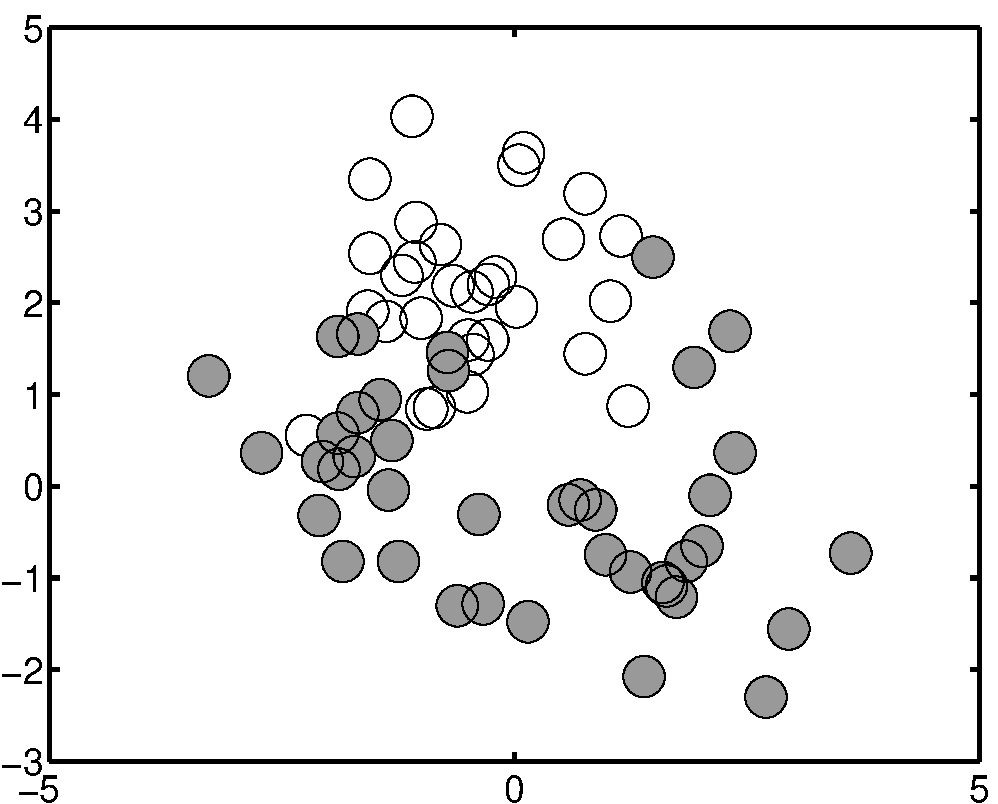
\includegraphics[width=0.7\linewidth]{class_data.pdf}
		\centering\caption{\label{fig:class_data}Some simple classification data}
	\end{figure}
\end{frame}

\begin{frame}
	\frametitle{Example - binary classification}
	\begin{figure}[tbh]
		\centering\includegraphics<1>[width=0.75\linewidth]{gpclass_hyp1_surf.pdf}
		\centering\includegraphics<2>[width=0.75\linewidth]{gpclass_hyp5_surf.pdf}
		\centering\includegraphics<3>[width=0.75\linewidth]{gpclass_hyp10_surf.pdf}
		\centering\caption{\label{fig:binary_results}Predictive probabilities averaged over 1000 Gibbs samples using an RBF covariance. As $\gamma$ is increased, the model overfits.}
	\end{figure}
\end{frame}

\begin{frame}
	\frametitle{Note}
	\begin{itemize}
		\item Inference:
			\begin{itemize}
				\item Gibbs sampling isn't the only option
				\item A popular alternative is Variational Bayes
			\end{itemize}
		\end{itemize}
\end{frame}

\begin{frame}
	\frametitle{Note 2 -- The Generative Process}
	\begin{itemize}
		\item Sometimes it's useful to think of the generative process defined by the model.
		\item In this case, to generate $N$ values of $y_n$ given the associated $x_n$:
		\begin{itemize}
			\item Sample $\blf$ from a \ac{GP} with mean $\mathbf{0}$ and Covariance matrix $\mathbf{C}$.
			\item For each $n=1\ldots N$:
			\begin{itemize}
				\item Sample $z_n\sim {\cal N}(f_n,1)$
				\item If $z_n>0$ set $y_n=1$, otherwise $y_n=0$.
			\end{itemize}
		\end{itemize}
		\item Some examples:
	\end{itemize}
	\begin{center}
		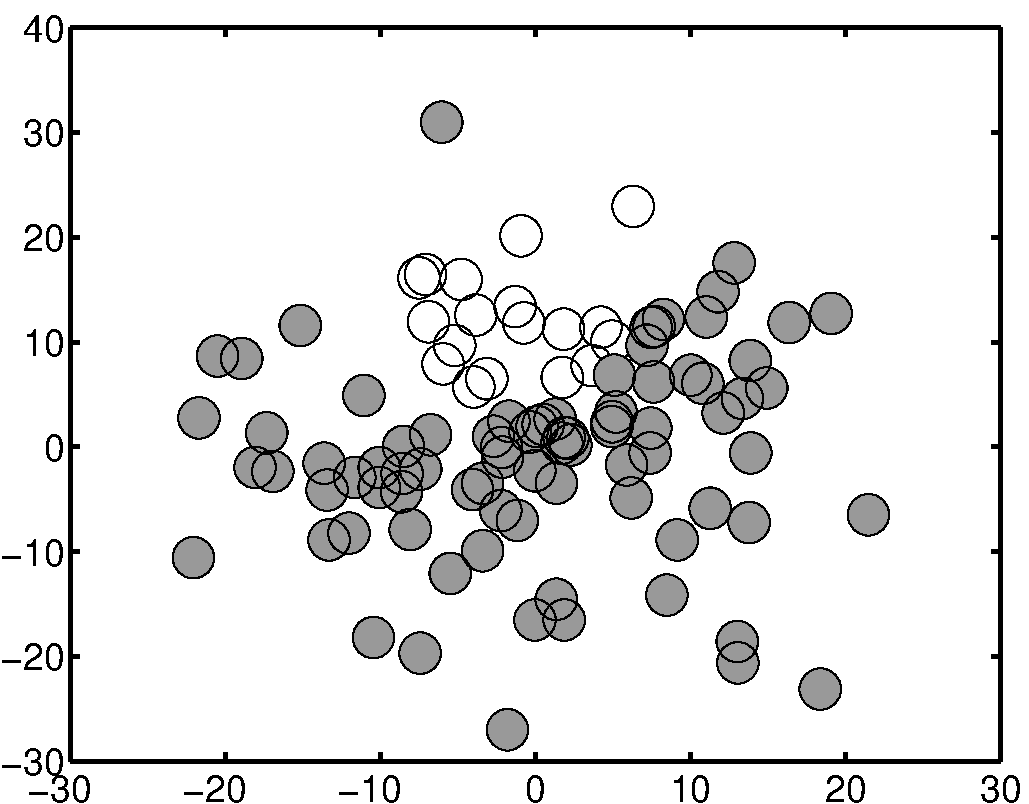
\includegraphics[width=0.3\linewidth]{gendata1.pdf}
		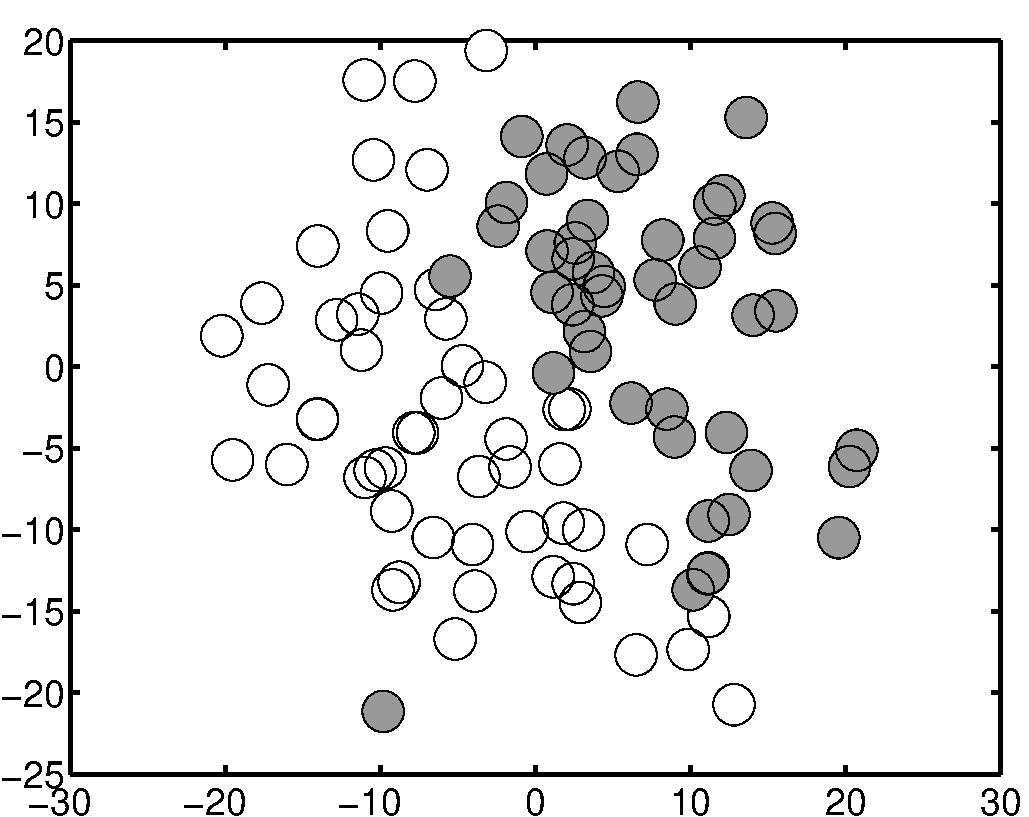
\includegraphics[width=0.3\linewidth]{gendata2.pdf}
		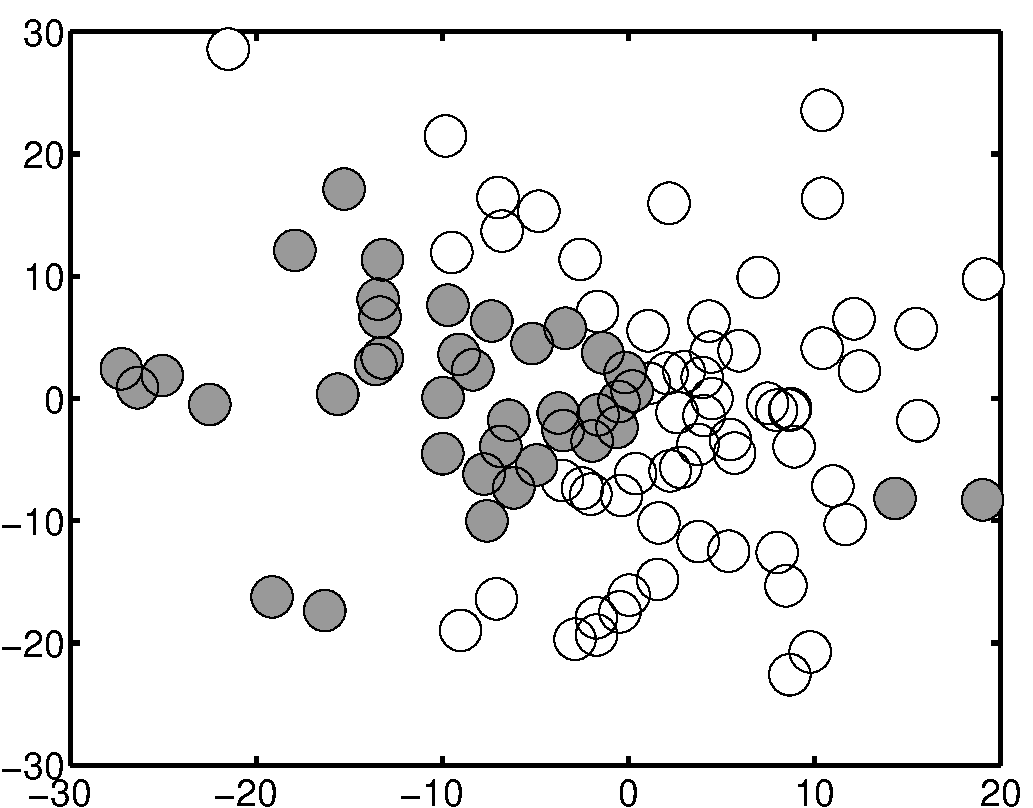
\includegraphics[width=0.3\linewidth]{gendata3.pdf}		
	\end{center}
\end{frame}

\begin{frame}
	\frametitle{A more general idea}
	\begin{itemize}
		\item Models of this form:
		\begin{itemize}
			\item $\blf \sim GP$
			\item $z_n\sim {\cal N}(f_n,1)$
			\item $P(y_n|z_n) = \delta(f(z_n))$
		\end{itemize}
		\item Can be used for more than just binary classification.
		\item<2-> Ordinal Regression:
			\begin{itemize}
				\item $P(y_n=k|z_n)$ is now chopped at both ends:
				\[
					P(y_n=k|z_n) = \delta(b_k<z_n<b_{k+1})
				\]
				\item Gibbs distribution for $z_n$ therefore involves a Gaussian truncated at both ends.
			\end{itemize}
		\item<3->As well as multi-class and semi-supervised classification\ldots
	\end{itemize}
\end{frame}


\begin{frame}
	\frametitle{Multi-class classification}
	\begin{itemize}
		\item The previous treatment can be extended to multiple classes.
		\item For a problem with $K$ classes:
		\begin{itemize}
			\item $K$ GP priors, $K$ $N$-dimensional latent vectors $\blf_k$.
			\item $N\times K$ auxiliary variables $z_{nk} \sim {\cal N}(f_{nk},1)$
			\item And:
			\[
				P(y_n=k|z_{n1},\ldots,z_{nK}) = \delta(z_{nk}>z_{ni} ~~\forall i\neq k)
			\]
		\end{itemize}
		\item<2->Gibbs sampling is similar to the binary case:
			\begin{itemize}
				\item Only tricky bit is efficently sampling from a $K$-dimensionl \ac{MVG} truncated such that the $k$th element is largest.
			\end{itemize}
		\item<3->Details of a Variational Bayes inference scheme in: \href{http://www.mitpressjournals.org/doi/pdf/10.1162/neco.2006.18.8.1790}{Girolami and Rogers 2006}

	\end{itemize}

\end{frame}

\begin{frame}
	\frametitle{Multi-class Example}
	\begin{figure}[tbh]
		\centering\includegraphics<1>[width=0.7\linewidth]{multiclass_data.pdf}
		\centering\includegraphics<2>[width=0.7\linewidth]{multiclass_k1.pdf}
		\centering\includegraphics<3>[width=0.7\linewidth]{multiclass_k2.pdf}
		\centering\includegraphics<4>[width=0.7\linewidth]{multiclass_k3.pdf}
		\centering\caption{\label{fig:multi-class}Multi-class classification example. RBF covariance, $\gamma=1$.}
	\end{figure}
\end{frame}

\begin{frame}
	\frametitle{Semi-supervised Classification}
	\begin{itemize}
		\item In some domains, only a subset of data are labeled [e.g. image classification]
		\begin{figure}[tbh]
			\centering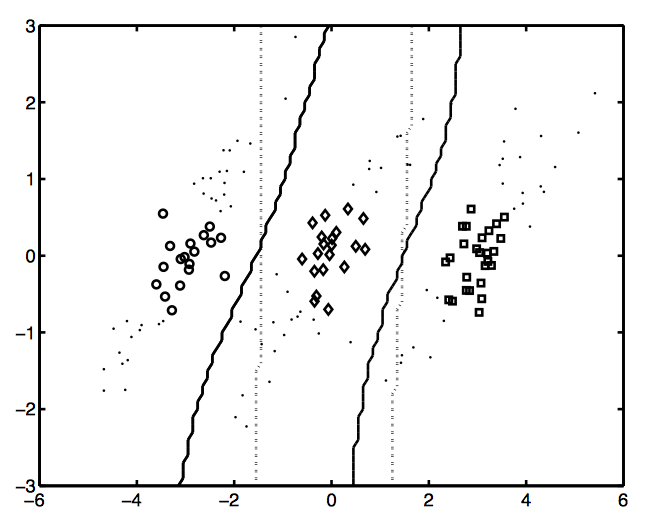
\includegraphics[width=0.5\linewidth]{semisup.png}
			\centering\caption{\label{fig:semisup}A toy semi-supervised classification problem.}
		\end{figure}
		\item Can be overcome using the \ac{NCNM} \href{http://papers.nips.cc/paper/2605-semi-supervised-learning-via-gaussian-processes.pdf}{Lawrence and Jordan 2004}
	\end{itemize}
\end{frame}

\begin{frame}
	\frametitle{The \ac{NCNM}}
	\begin{itemize}
		\item Going back to binary classification, the auxiliary variable trick can be visualised:
		\begin{figure}[tbh]
			\centering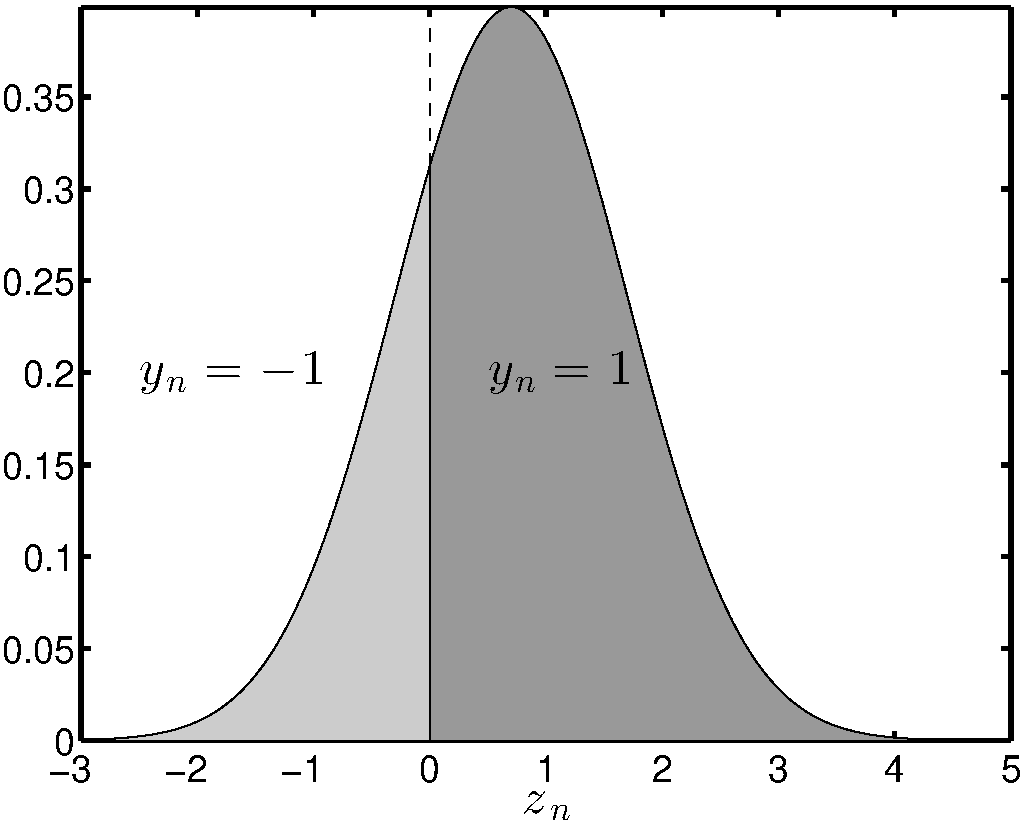
\includegraphics[width=0.7\linewidth]{vis_aux.pdf}
			\centering\caption{\label{fig:vis_aux}Visualisation of the auxiliary variable trick. The Gaussian has mean $f_n$. Note that I'm not calling the classes $\pm 1$.}
		\end{figure}
	\end{itemize}
\end{frame}

\begin{frame}
	\frametitle{The \ac{NCNM}}
	\begin{itemize}
		\item To include unlabeled data, we add a third category, for $y_n=0$:
		\begin{figure}[tbh]
			\centering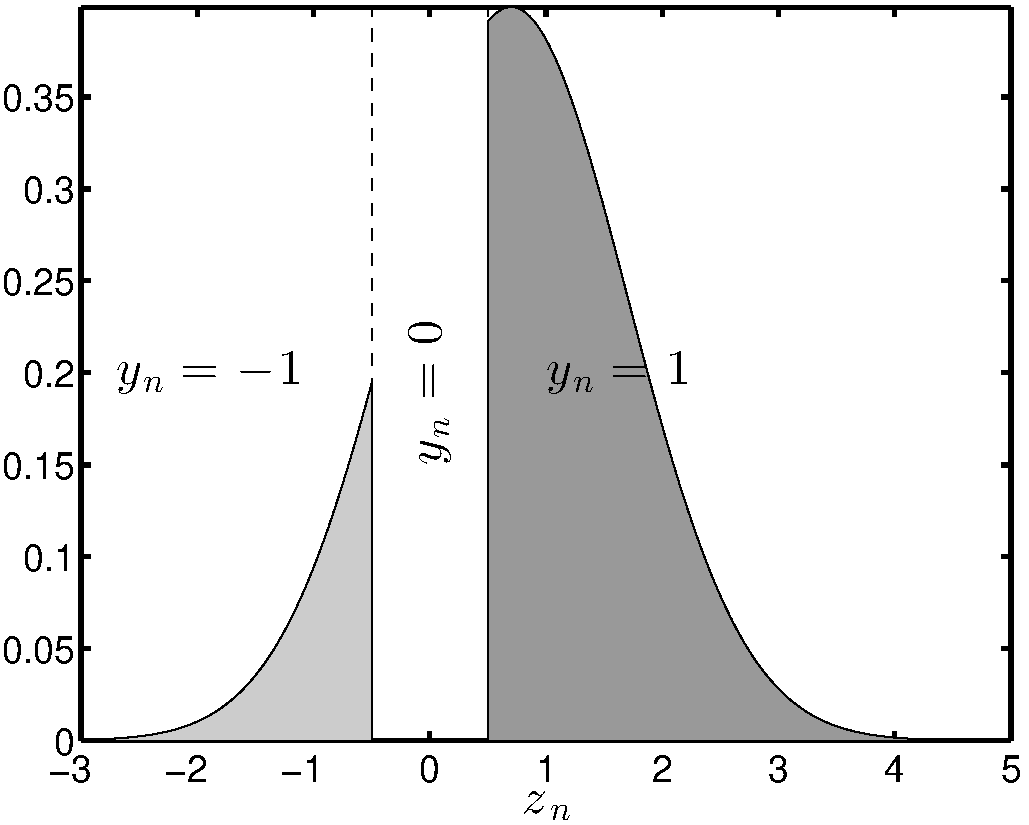
\includegraphics[width=0.5\linewidth]{vis_aux_ncnm.pdf}
			\centering\caption{\label{fig:vis_aux_ncnm}Visualisation of the \ac{NCNM} with a null region of width 1.}
		\end{figure}
		\[
			p(y_n|z_n) = \left\{ 
				\begin{array}{ll}
					\delta(z_n<-a) & y_n = -1\\
					\delta(z_n>a) & y_n = 1\\
					\delta(z_n>-a) - \delta(z_n>a) & y_n=0
				\end{array}
			\right.
		\]
	\end{itemize}
\end{frame}

\begin{frame}
	\frametitle{The \ac{NCNM}}
	\begin{itemize}
		\item The final step is to introduce another set of latent variables.
		\begin{itemize}
			\item $g_n=0$ if $y_n$ is observed (i.e. labeled) and $g_n=1$ otherwise.
		\end{itemize}
		\item And enforce the constraint that no unlabeled points can exist in the null region:
		\[
			P(y_n=0|g_n=1) = 0
		\]
		\item<2->This has the effect of introducing an empty region around the decision boundary
		\begin{itemize}
			\item i.e. pushing the decision boundary into regions of empty space
		\end{itemize}
		\item<3->Inference:
		\begin{itemize}
			\item Gibbs sampling is the same as the binary case except $z_n|f_n,g_n=1$.
			\item This is a mixture of two truncated Gaussians -- sample the component, and then sample $z_n$.
		\end{itemize}
	\end{itemize}
\end{frame}

\begin{frame}
	\frametitle{NCNM Example}
	\begin{figure}[tbh]
		\centering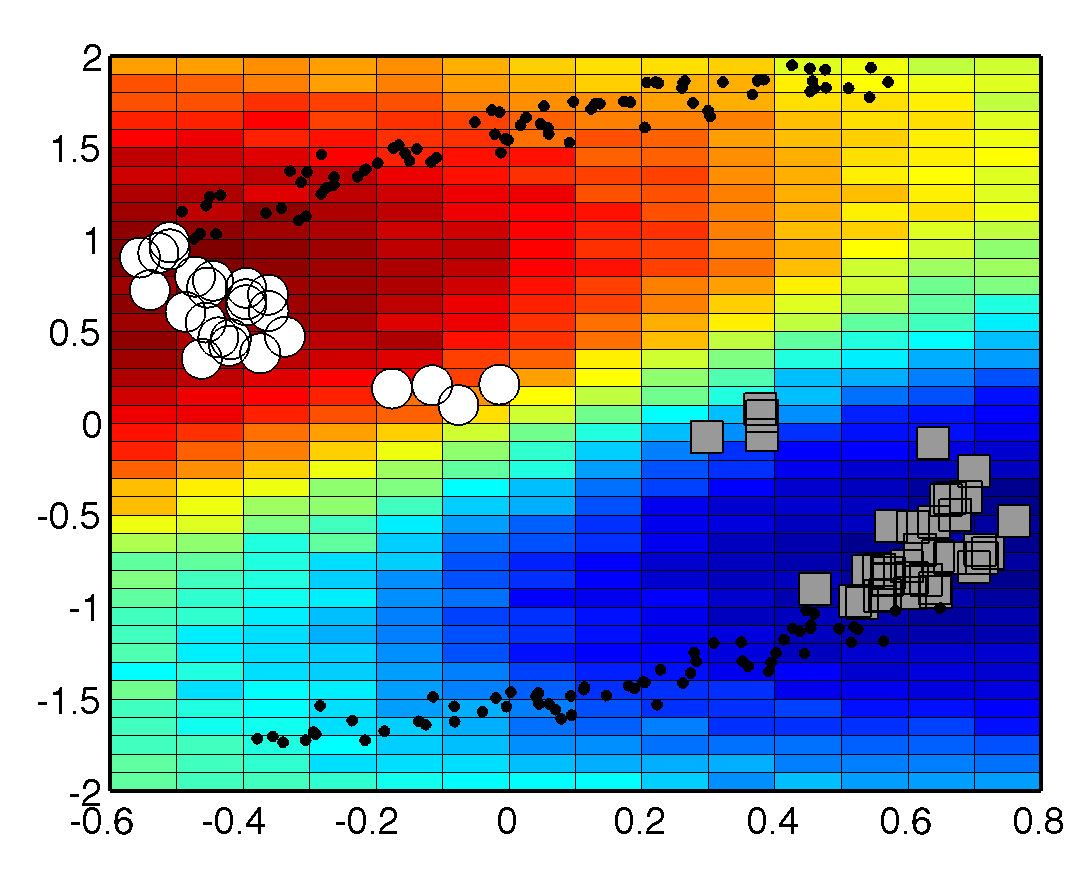
\includegraphics[width=0.8\linewidth]{ncnm_a0.pdf}
		\centering\caption{\label{fig:ncnm_a0}Standard GP classification (unlabeled data ignored)}
	\end{figure}
\end{frame}

\begin{frame}
	\frametitle{NCNM Example}
	\begin{figure}[tbh]
		\centering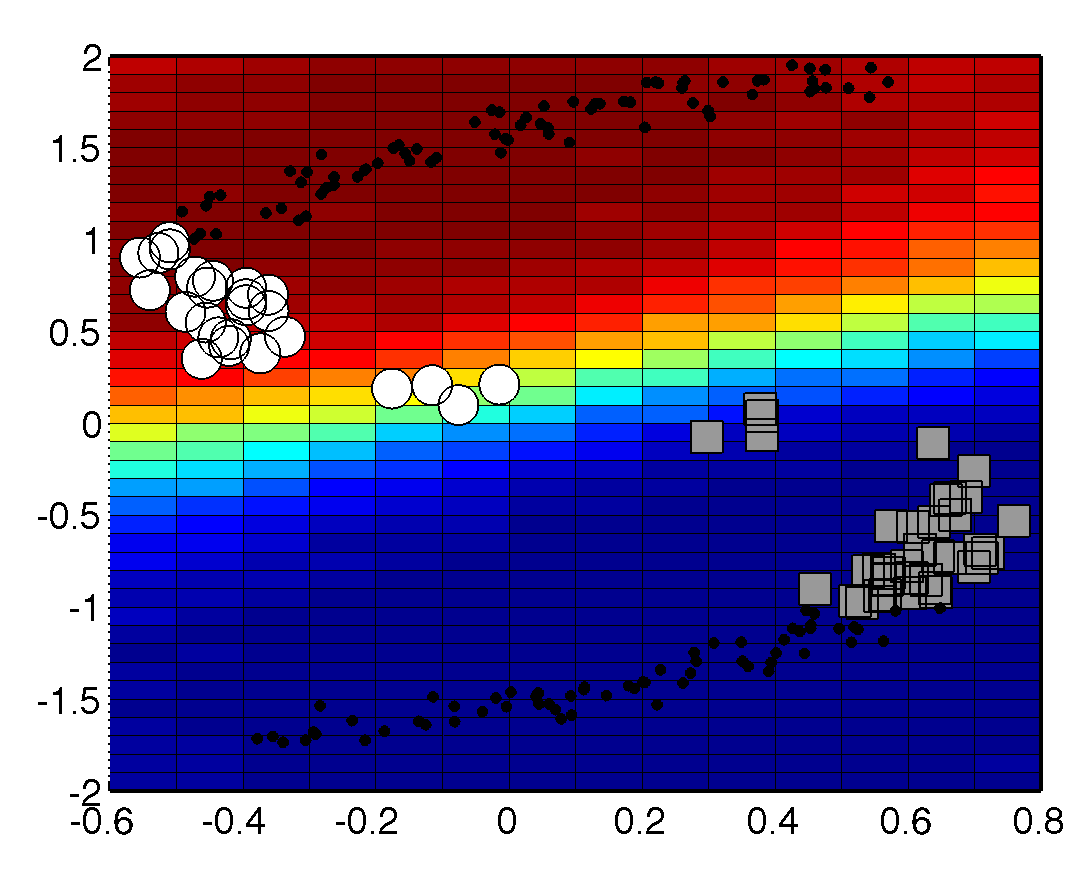
\includegraphics[width=0.8\linewidth]{ncnm_a05.pdf}
		\centering\caption{\label{fig:ncnm_a0.5}NCNM GP classification}
	\end{figure}
\end{frame}

\begin{frame}
	\frametitle{Multi-class \ac{NCNM}}
	\begin{itemize}
		\item This idea can be extended to the multi-class setting.
		\item See \href{http://jmlr.org/proceedings/papers/v1/rogers07a/rogers07a.pdf}{Rogers and Girolami 2007}
	\end{itemize}
		{\small \[
		P(y_n=k|z_{n1},\ldots,z_{nK}) = \left \{
				\begin{array}{cc}
					\delta(z_{nk} > z_{ni} + a~~\forall i \neq k) & y_n>0\\
					1 - \sum_j \delta(z_{nj} > z_{ni} + a ~~\forall i \neq j) & y_n=0
				\end{array}
			\right.
		\]}
		\begin{figure}[tbh]
			\centering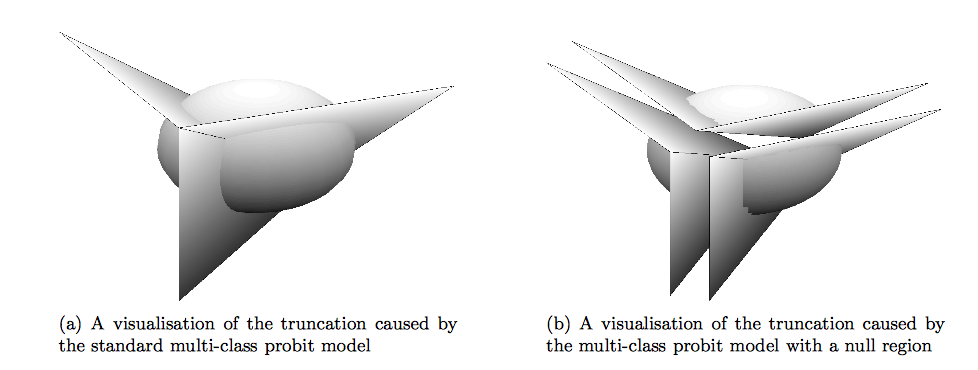
\includegraphics[width=\linewidth]{nullsphere.png}
			\centering\caption{\label{fig:nullsphere}Visualisation of truncation}
		\end{figure}
\end{frame}

\begin{frame}
	\frametitle{Summary}
	\begin{itemize}
		\item \ac{GP} priors aren't restricted to regression.
		\item Analytical solutions aren't possible
		\item Auxiiliary Variable Trick makes inference (via Gibbs sampling or Variational Bayes) straightforward for:
		\begin{itemize}
			\item Binary classification
			\item Ordinal regression
			\item Multi-class classification
			\item Semi-supervised classification (binary and mutli-class)
			\item As well as others (e.g. binary PCA)
		\end{itemize}
	\end{itemize}
\end{frame}
